\section{Adaptive Q-Band Suppression Controller}




\subsection{Tractor Prediction Model and ESO}
The online optimizer uses a low-dimensional tractor-side nonlinear prediction model. Trailer force, liquid sloshing, tire mismatch, road slope, and parameter errors are not explicit states; they are collected as residual terms. Let $v_x$, $v_y$, $r$, and $\delta$ denote tractor longitudinal speed, lateral speed, yaw rate, and front-wheel steering angle. With front and rear cornering stiffnesses $C_f$ and $C_r$, the tire slip angles and lateral forces are
\begin{equation}
    \alpha_f=\delta-\frac{v_y+l_fr}{v_x},\qquad
    \alpha_r=-\frac{v_y-l_rr}{v_x},
\end{equation}
\begin{equation}
    F_{yf}=C_f\alpha_f,\qquad F_{yr}=C_r\alpha_r ,
\end{equation}
where $l_f$ and $l_r$ are the distances from tractor center of gravity to the front and rear axles. The nominal prediction model is
\begin{equation}
\begin{aligned}
    \dot v_y &= \frac{F_{yf}\cos\delta+F_{yr}}{m_{\mathrm{eq}}}-v_xr+d_y,\\
    \dot r &= \frac{l_fF_{yf}\cos\delta-l_rF_{yr}}{I_{z,\mathrm{eq}}}+d_r ,
\end{aligned}
\label{eq:tractor_2dof}
\end{equation}
where $m_{\mathrm{eq}}$ and $I_{z,\mathrm{eq}}$ are the hitch-angle-scheduled equivalent lateral mass and yaw inertia, and $d_y,d_r$ are lumped lateral and yaw residuals. The lateral acceleration used by Q-band is computed from the prediction model as
\begin{equation}
    a_{y,k}^{\mathrm{pred}}=\dot v_{y,k}+v_{x,k}r_k .
    \label{eq:ay_prediction}
\end{equation}

An extended-state observer (ESO) estimates the yaw-channel residual:
\begin{equation}
\begin{aligned}
    \dot{\hat r} &= \frac{l_f\hat F_{yf}\cos\delta-l_r\hat F_{yr}}{I_{z,\mathrm{eq}}}
    +\hat d_r+\beta_{r1}(r-\hat r),\\
    \dot{\hat d}_r &= \beta_{r2}(r-\hat r),
\end{aligned}
\label{eq:eso_full}
\end{equation}
where $\hat r$ and $\hat d_r$ are the estimated yaw rate and yaw residual, and $\beta_{r1},\beta_{r2}>0$ are observer gains. The lateral residual is obtained from the difference between the measured lateral acceleration and the kinematic centripetal component:
\begin{equation}
    \hat d_y = a_y^{\mathrm{centri}}-a_y^{\mathrm{meas}}
    = v_x r-(a_y^{\mathrm{imu}}-\Delta a_{y,0}),
    \label{eq:lateral_residual}
\end{equation}
where $a_y^{\mathrm{imu}}$ is the IMU lateral acceleration, $\Delta a_{y,0}$ is its slowly updated zero offset, and $a_y^{\mathrm{centri}}=v_xr$ is the low-dimensional centripetal estimate. In the prediction horizon, the residual is held or decayed as
\begin{equation}
    \hat d_{\ell|k}=\lambda_d^\ell \hat d_k,\qquad 0<\lambda_d\leq1,
    \label{eq:eso_decay}
\end{equation}
where $\ell$ is the prediction step and $\lambda_d$ is the residual forgetting factor.

\subsection{Hitch-Angle and Equivalent Inertia}
\label{equivalent_inertia_hitch_angle}
The equivalent parameters in \eqref{eq:tractor_2dof} use a tractor-trailer articulation prior. Let the tractor and trailer headings be $\psi_1$ and $\psi_2$, and define the hitch angle as
\begin{equation}
    \gamma=\psi_1-\psi_2 .
\end{equation}
With measured tractor yaw rate $r_m$, the trailer heading and hitch angle are estimated by
\begin{equation}
\begin{aligned}
    \dot{\hat\psi}_2 &=
    K_v\frac{v_x}{L_2}\left(\frac{L_h}{L_1}\tan\delta\cos\hat\gamma+\sin\hat\gamma\right),\\
    \dot{\hat\gamma} &= r_m-\dot{\hat\psi}_2 .
\end{aligned}
\label{eq:hitch_estimator}
\end{equation}
Here $L_1$ is the tractor wheelbase, $L_2$ is the distance from the hitch to the trailer axle group, and $L_h$ is the distance from the tractor rear axle to the hitch. The correction factor
\begin{equation}
    K_v=1-\frac{m_2v_x^2e}{L_1L_2k_3}
    \label{eq:hitch_ckds}
\end{equation}
approximates trailer-axle sideslip, where $m_2$ is trailer mass, $e$ is the equivalent hitch-to-trailer geometric offset, and $k_3$ is the trailer axle cornering stiffness. When these trailer tire parameters are not available, $K_v=1$ is used.

The trailer contribution is projected into tractor lateral inertia and yaw inertia:
\begin{equation}
    m_{x,\mathrm{eq}}(\hat\gamma)=m_1+m_2\cos^2\hat\gamma,\qquad
    m_{y,\mathrm{eq}}(\hat\gamma)=m_1+m_2\sin^2\hat\gamma,
    \label{eq:eq_mass}
\end{equation}
\begin{equation}
    I_{z,\mathrm{eq}}(\hat\gamma)=I_{z1}
    +I_{z2}\left(\frac{d_1}{d_2}\right)^2\cos^2\hat\gamma
    +m_2d_1^2\sin^2\hat\gamma .
    \label{eq:eq_inertia}
\end{equation}
Here $m_1$ is tractor mass, $I_{z1}$ and $I_{z2}$ are tractor and trailer yaw inertias, and $d_1,d_2$ are the equivalent geometric distances used to project trailer yaw inertia to the tractor yaw axis. In the NMPC model, $m_{\mathrm{eq}}=m_{y,\mathrm{eq}}(\hat\gamma)$, and $I_{z,\mathrm{eq}}$ is evaluated from \eqref{eq:eq_inertia}, after low-pass filtering, upper/lower saturation, and rate limiting.

\subsection{Band-Energy Projection}
Let the prediction horizon contain $N$ samples with sampling time $\Delta t$. The predicted lateral-acceleration sequence is
\begin{equation}
    \mathbf{A}_y=[a_{y,0},a_{y,1},\ldots,a_{y,N-1}]^\T ,
\end{equation}
where $a_{y,k}$ is computed from \eqref{eq:ay_prediction} for a dynamic predictor, or from $a_{y,k}\approx v_{x,k}^2\kappa_k$ for a kinematic predictor with path curvature $\kappa_k$. For a critical band $\mathcal{B}_i=[f_i^-,f_i^+]$, choose discrete frequencies $f_{ij}$ and time grid $t_k=k\Delta t$. Define
\begin{equation}
    \mathbf{c}_{ij}=[\cos(2\pi f_{ij}t_0),\ldots,\cos(2\pi f_{ij}t_{N-1})]^\T ,
\end{equation}
\begin{equation}
    \mathbf{s}_{ij}=[\sin(2\pi f_{ij}t_0),\ldots,\sin(2\pi f_{ij}t_{N-1})]^\T .
\end{equation}
The predicted energy in the $i$th band is
\begin{equation}
    E_i(\mathbf{A}_y)=\mathbf{A}_y^\T\mathbf{Q}_i\mathbf{A}_y,
\end{equation}
\begin{equation}
    \mathbf{Q}_i=\frac{1}{N^2}\sum_j(\mathbf{c}_{ij}\mathbf{c}_{ij}^\T+\mathbf{s}_{ij}\mathbf{s}_{ij}^\T)\succeq0 .
\end{equation}
The matrix $\mathbf{Q}_i$ is precomputed from $\Delta t$, $N$, and $\mathcal{B}_i$. It adds no vehicle state and only projects $\mathbf{A}_y$ onto dangerous frequency components.

\begin{figure*}[!t]
\centering
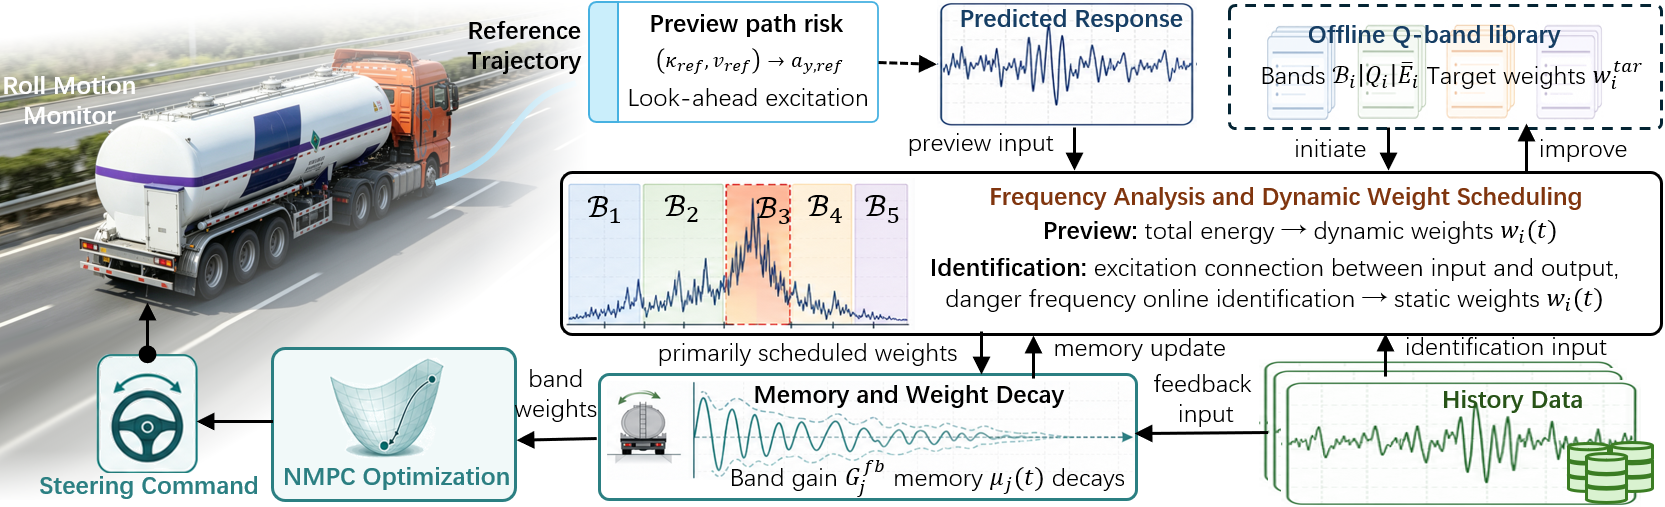
\includegraphics[width=0.98\textwidth]{fig/qband_scheduler.png}
\caption{Adaptive Q-band scheduling. Preview risk raises the band weights before aggressive path segments, while feedback monitoring strengthens dynamically amplified bands and delays weight release after residual sloshing.}
\label{fig:qband_scheduler}
\end{figure*}



\subsection{Optimization Problem}
Let $\mathbf{x}_k$ be the prediction state, $u_k=\delta_{\mathrm{cmd},k}$ the steering command, $\mathbf{U}=[u_0,\ldots,u_{N-1}]^\T$, and $\mathbf{S}=[s_1,\ldots,s_{n_b}]^\T$ the nonnegative slack variables for $n_b$ Q-bands. The Q-band ART objective is
\begin{equation}
\begin{aligned}
\min_{\mathbf{U},\mathbf{S}}~&
J_{\mathrm{trk}}+J_u+J_{\Delta u}
+w_a\|\mathbf{A}_y\|_2^2+w_1\|\mathbf{D}_1\mathbf{A}_y\|_2^2\\
&+w_2\|\mathbf{D}_2\mathbf{A}_y\|_2^2
+\sum_{i=1}^{n_b} w_i(t)\mathbf{A}_y^\T\mathbf{Q}_i\mathbf{A}_y
+\sum_{i=1}^{n_b}\rho_i s_i^2 .
\end{aligned}
\label{eq:qband_cost}
\end{equation}
Here $J_u=w_u\|\mathbf{U}\|_2^2$, $J_{\Delta u}=w_{\Delta u}\|\mathbf{D}_u\mathbf{U}\|_2^2$, and $w_a,w_1,w_2,\rho_i$ are positive tuning weights. The first- and second-order difference matrices are calculated by
\begin{equation}
    (\mathbf{D}_1\mathbf{A}_y)_k
    =\frac{a_{y,k+1}-a_{y,k}}{\Delta t},
\end{equation}
\begin{equation}
    (\mathbf{D}_2\mathbf{A}_y)_k
    =\frac{a_{y,k+2}-2a_{y,k+1}+a_{y,k}}{\Delta t^2}.
\end{equation}
The tracking cost uses the previewed reference position and heading:
\begin{equation}
    J_{\mathrm{trk}}=w_{xy}(\|\mathbf{X}-\mathbf{X}_{\mathrm{ref}}\|_2^2
    +\|\mathbf{Y}-\mathbf{Y}_{\mathrm{ref}}\|_2^2)
    +w_{\psi}\|\boldsymbol{\psi}-\boldsymbol{\psi}_{\mathrm{ref}}\|_2^2 ,
\end{equation}
where $\mathbf{X}$, $\mathbf{Y}$, and $\boldsymbol{\psi}$ collect predicted tractor positions and headings over the horizon, and the subscript ``ref'' denotes the path-preview sequence.

The constraints are
\begin{equation}
\begin{aligned}
    \mathbf{x}_{k+1}&=f(\mathbf{x}_k,u_k,\hat d_{k|k},m_{\mathrm{eq}},I_{z,\mathrm{eq}}),\\
    |a_{y,k}|&\leq a_{y,\max}^{\mathrm{dyn}},\\
    u_{\min}&\leq u_k\leq u_{\max},\quad |\Delta u_k|\leq \Delta u_{\max},\\
    E_i(\mathbf{A}_y)&\leq \bar{E}_i+s_i,\quad s_i\geq0 .
\end{aligned}
\label{eq:qband_constraints}
\end{equation}
The bound $a_{y,\max}^{\mathrm{dyn}}$ is the speed- and risk-dependent lateral-acceleration limit, and $\bar E_i$ is the calibrated safe energy threshold of band $\mathcal{B}_i$.

\subsection{Preview-Adaptive Scheduling}
Q-band ART uses preview risk as the main trigger, and the complete weight-scheduling logic is summarized in Fig.~\ref{fig:qband_scheduler}. The reference lateral-acceleration sequence $\mathbf{A}_{y,\mathrm{ref}}$ is computed from future path curvature as
\begin{equation}
    a_{y,\mathrm{ref},k}=v_{x,k}^2\kappa_{\mathrm{ref},k},
    \qquad
    \kappa_{\mathrm{ref},k}\approx
    \frac{\mathrm{wrap}(\psi_{\mathrm{ref},k+1}-\psi_{\mathrm{ref},k})}{\Delta s_k},
\end{equation}
where $\Delta s_k$ is the preview arc-length interval and $\mathrm{wrap}(\cdot)$ keeps heading differences within $[-\pi,\pi]$. The preview risk in band $i$ is
\begin{equation}
    R_i^{\mathrm{pre}}=\left[
    \frac{\mathbf{A}_{y,\mathrm{ref}}^\T\mathbf{Q}_i\mathbf{A}_{y,\mathrm{ref}}}
    {\bar{E}_{i,\mathrm{ref}}}-1\right]_+ ,
    \label{eq:preview_risk}
\end{equation}
where $[x]_+=\max(x,0)$ and $\bar{E}_{i,\mathrm{ref}}$ is the preview activation threshold. The preview-only activation is
\begin{equation}
    \lambda_i^{\mathrm{pre}}=1-\exp(-\kappa_{\mathrm{pre}}R_i^{\mathrm{pre}}),
\end{equation}
where $\kappa_{\mathrm{pre}}>0$ controls how quickly the weight rises before an aggressive maneuver.


\subsection{Feedback Band Monitoring and Residual Sloshing Memory}
Preview alone cannot identify bands that become dangerous due to loading, fill level, tire state, or unmodeled trailer dynamics. A feedback monitor is therefore added to detect bands with non-negligible input and amplified measured output. Over a sliding window of $M$ samples, define
\begin{equation}
    \mathbf{a}_M(t)=[a_y^{\mathrm{mon}}(t-M+1),\ldots,a_y^{\mathrm{mon}}(t)]^\T ,
\end{equation}
where $a_y^{\mathrm{mon}}$ is the measured or predicted lateral acceleration after offset correction. The monitored output is
\begin{equation}
    y^{\mathrm{mon}}\in\{r-\hat r,\; a_y^{\mathrm{imu}}-a_y^{\mathrm{pred}},\; \dot\phi\},
\end{equation}
with the output window
\begin{equation}
    \mathbf{y}_M(t)=[y^{\mathrm{mon}}(t-M+1),\ldots,y^{\mathrm{mon}}(t)]^\T .
\end{equation}
The yaw and acceleration residuals are available from tractor-side sensing, and roll rate $\dot\phi$ is used when a roll sensor is available. For a monitoring band $\mathcal{C}_j$, construct $\mathbf{Q}_j^{M}$ as $\mathbf{Q}_i$ but with window length $M$. The input and output band energies are
\begin{equation}
    E_{a,j}^{\mathrm{fb}}=\mathbf{a}_M^\T\mathbf{Q}_j^{M}\mathbf{a}_M,\qquad
    E_{y,j}^{\mathrm{fb}}=\mathbf{y}_M^\T\mathbf{Q}_j^{M}\mathbf{y}_M ,
\end{equation}
and the observed amplification is
\begin{equation}
    G_j^{\mathrm{fb}}=\sqrt{\frac{E_{y,j}^{\mathrm{fb}}}{E_{a,j}^{\mathrm{fb}}+\epsilon}},
    \label{eq:feedback_gain}
\end{equation}
where $\epsilon$ avoids division by zero. A dynamically dangerous band must satisfy both non-negligible input and amplified output:
\begin{equation}
    R_j^{\mathrm{fb}}=
    \left[\frac{E_{a,j}^{\mathrm{fb}}}{\bar E_{a,j}}-1\right]_+
    \left[\frac{G_j^{\mathrm{fb}}}{\bar G_{j}^{\mathrm{fb}}}-1\right]_+ .
    \label{eq:feedback_risk}
\end{equation}
Here $\bar E_{a,j}$ is the minimum input-energy threshold, and $\bar G_j^{\mathrm{fb}}$ is the nominal amplification level from calibration or low-risk data.

To retain residual sloshing after steering input decreases, the feedback risk is stored as
\begin{equation}
    \mu_j(t)=\max\{\lambda_m\mu_j(t-\Delta t),~R_j^{\mathrm{fb}}(t)\},\qquad 0<\lambda_m<1 ,
\end{equation}
where $\lambda_m$ is the memory decay factor. If the monitoring bands $\mathcal{C}_j$ are finer than the default controller bands $\mathcal{B}_i$, the feedback memory is mapped to the controller band by the overlap ratio
\begin{equation}
    \mu_i^{\mathrm{dyn}}(t)=\max_j \sigma_{ij}\mu_j(t),\qquad
    \sigma_{ij}=\frac{|\mathcal{B}_i\cap\mathcal{C}_j|}{|\mathcal{B}_i|}.
\end{equation}
Thus, bands observed to be both excited and amplified increase the default Q-band weights.

The preview and feedback activations are fused before filtering:
\begin{equation}
    \lambda_i(t)=1-\exp[-\kappa_{\mathrm{pre}}R_i^{\mathrm{pre}}-\kappa_{\mathrm{fb}}\mu_i^{\mathrm{dyn}}(t)],
\end{equation}
\begin{equation}
    w_{i,\mathrm{tar}}^{\mathrm{dyn}}(t)=
    \min\{w_i^{\max},~w_i^{\mathrm{tar}}(1+\eta_{\mathrm{fb}}\mu_i^{\mathrm{dyn}}(t))\},
\end{equation}
\begin{equation}
    w_i^{\mathrm{raw}}(t)=w_i^{\min}
    +\lambda_i(t)\left(w_{i,\mathrm{tar}}^{\mathrm{dyn}}(t)-w_i^{\min}\right).
    \label{eq:raw_weight_combined}
\end{equation}
Here $\kappa_{\mathrm{fb}}$ and $\eta_{\mathrm{fb}}$ tune the feedback contribution, $w_i^{\min}$ is the low-risk weight, $w_i^{\mathrm{tar}}$ is the nominal calibrated target weight, and $w_i^{\max}$ prevents excessive conservatism. Finally, a non-symmetric filter is applied:
\begin{equation}
    w_i(t)=(1-\alpha_i)w_i(t-\Delta t)+\alpha_i w_i^{\mathrm{raw}}(t),
\end{equation}
where $\alpha_i=\alpha_\uparrow$ when $w_i^{\mathrm{raw}}>w_i(t-\Delta t)$ and $\alpha_i=\alpha_\downarrow$ otherwise, with $\alpha_\uparrow>\alpha_\downarrow$. This makes the weight rise quickly when preview or feedback detects risk, and decay slowly while residual sloshing memory remains.

% \subsection{Implementation Notes}
% The Q-band module is model-agnostic. For a kinematic predictor, $a_{y,k}$ can be approximated from curvature or steering; for a dynamic predictor, it can be computed from $\dot v_y+v_xr$; for high-fidelity TruckSim validation, it is evaluated from the predicted tracking response. In all cases, the controller suppresses the lateral excitation sequence rather than explicitly controlling the liquid state.
